
%(BEGIN_QUESTION)
% Copyright 2011, Tony R. Kuphaldt, released under the Creative Commons Attribution License (v 1.0)
% This means you may do almost anything with this work of mine, so long as you give me proper credit

Suppose the following solenoid-controlled valve system is functioning as it is designed to, under regular operating conditions (i.e. no emergencies, no abnormal circumstances).  The pressure inside the process vessel registers a steady 75 PSI on the pressure gauge (PG), and the pneumatically-operated valve PCV-5 is an ``air-to-open'' design:

$$\includegraphics[width=15.5cm]{i00299x01.eps}$$

\noindent
Choose the best answer describing the immediate effect on this process if solenoid valve SOV-2 suddenly suffers an ``open'' electrical fault in its coil:

\begin{itemize}
\item{} The vessel will immediately implode due to a rapid decrease in internal gas pressure
\vskip 10pt
\item{} The process vessel pressure will begin to rise as PCV-5 shuts off and traps gas
\vskip 10pt
\item{} The process vessel pressure will begin to drop as PCV-5 vents gas to atmosphere
\vskip 10pt
\item{} The process will continue to operate normally, maintaining 75 PSI in the vessel
\end{itemize}

\underbar{file i00299}
%(END_QUESTION)





%(BEGIN_ANSWER)

The process will continue to operate normally, maintaining 75 PSI in the vessel

%(END_ANSWER)





%(BEGIN_NOTES)

{\bf This question is intended for exams only and not worksheets!}.

%(END_NOTES)


